\chapter{Background}
\label{cha:LiteratureReview}

The chapter explains aspects required to fully comprehend the project's achievements alongside an evaluation of current literature and the respective gaps.

The chapter contains the following sections:

\begin{itemize}
    \item \textbf{Project context} \\ 
    Provides the user with the base knowledge required to understand the context and purpose of the following literature review.
    
    \item \textbf{Literature Review} \\
    A review of currently available literature on relevant topics. Recommendations and research gaps are identified and discussed.

\end{itemize}

\section{Project context}

To fully understand the literature review, it is necessary to introduce and explain the base knowledge before continuing.

\subsection{Public-key Cryptography and Key Exchange}

Asymmetric cryptography facilitates the secure encryption of messages in end-to-end encryption (E2EE), verification of digital signatures, and sharing of pre-communication secrets, among others. 

The asymmetry stems from the use of "Public" and "Private" keys. The public-key is used to encrypt data that only the respective private-key can decrypt. Hence, this means that sharing the keys required to encrypt can be performed across insecure channels.

An E2EE connection uses the key types discussed previously to exchange messages between verified parties securely. However, this hinges on the verification of the initial parties, if one party impersonates another and receives sensitive communication, the secure encryption is completely circumvented. Therefore, the correct identification of parties is crucial to maintaining security. The exploitation of this is known as a Man-in-the-middle (MiTM) attack. This attack is commonly bidirectional, and if executed correctly, there is often no discerning change to the user experience. Figure \ref{fig:mitm} contains a visual representation of this attack. In the diagram Eve (attacker) is impersonating Alice to Bob and Bob to Alice. Therefore, as both directions of communication are compromised all traffic will route through the attacker Eve.

\begin{center}
    \newcommand{\tgap}{0.1cm}
	\begin{tikzpicture}[
		every node/.style={fill=white},
		diagram item/.style={},
		align=left
	]         

	\node (Router)[
		diagram item,
		label=above:Alice,
		yshift=-2cm
	] {
\includegraphics[scale=\ciscoImageScale]{\cisco/workstation}};

	\node (Victim)[
		diagram item,
		label=above:Bob,
		right of=Router,
		xshift=7cm
	] {
\includegraphics[scale=\ciscoImageScale]{\cisco/workstation}};

	\coordinate (CENTER) at ($(Victim)!0.5!(Router)$);
	\node (Attacker)[
		label=below:Eve,
		below of=CENTER,
		yshift=-3.5cm
	] {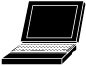
\includegraphics[scale=\ciscoImageScale]{\cisco/laptop}};

	\draw[-] (Router)--node[yshift=0.5cm]{Old Connection}(Victim);
	\draw[red, very thick] (Router)--node{New Connection}(Attacker);
	\draw[red, very thick] (Attacker)--node{New Connection}(Victim);
\end{tikzpicture} 

    \begin{figure}[h]
        \caption{Photo depicting a MITM attack}
        \label{fig:mitm}
    \end{figure}
\end{center}

Due to the assumption that the attacking party (Eve) does not have the same public-private key pair as either party (Alice or Bob), the unique aspects of the keys can be used to identify parties. This is achieved succinctly through the use of a fingerprint. A fingerprint is a string of alphanumerical characters that are unique to each key. Therefore the fingerprint of the two respective public keys are different, and, thus can be used for identification. There are, however, issues in how a user should link a key's fingerprint to an identity. One example way to achieve this is by meeting in-person to exchange fingerprints. This paper will, however, assume that users have been through this process.

The fingerprint of the key is generated by running the main key components through a secure one-way hash function such as SHA-256. This process produces a digest of a fixed length that can be used to compare keys. Therefore, the comparison of expected and actual fingerprints can be used to detect MiTM attacks.

Historically fingerprints have been represented as a hexadecimal string, whereon verification fingerprints are compared between two substrates, for example, a monitor screen and a business card. Figure \ref{fig:businessCard} shows an example business card. A user will then use the fingerprint present on the card to compare to the one available on a device. This will have to be performed by each user. This process is known as the \textit{``authentication ceremony.''} 

\begin{figure}[h!]
    \centering
    \fbox{
        %%% BUSINESS CARD SIZE
\newlength{\cardw}
\newlength{\cardh}
%% My size
\setlength{\cardw}{90mm}
\setlength{\cardh}{50mm}

%% ISO 7810 size: 85.60mm × 53.98mm
% \setlength{\cardw}{85.60mm}
% \setlength{\cardh}{53.98mm}

%% European size: 85mm × 55mm
% \setlength{\cardw}{85mm}
% \setlength{\cardh}{55mm}

%% US size: 3.5 in × 2 in
% \setlength{\cardw}{3.5in}
% \setlength{\cardh}{2in}


%%% DEFINE USER DATA
\newcommand{\Name}{
	{\huge \textbf{John Doe} }
}%
\newcommand{\Description}{
	{\large Linux System Administrator }
}%
\newcommand{\Email}{
	{\large john@example.com }
}%
\newcommand{\Phone}{
	{\large +1 234 56 78 910 }
}%
\newcommand{\Site}{
	{\large johndoe.com }
}%

\newcommand{\FingerprintOne}{
    {\footnotesize 6424 AD56 4BF7 06BC 0696
     }
}%
\newcommand{\FingerprintTwo}{
    {\footnotesize BC61 412A 20D9 2450 BDE8}
}%

\definecolor{mycolor}{rgb}{0.427,0.592,0.749} % RGB(109,151,191)

\begin{tikzpicture}

% card content
\foreach \i in {0} \foreach \j in {0} {
   \node[black!25!mycolor][right] at (\i*\cardw+0.05\cardw,\j*\cardh+0.85\cardh) {\Name};
   \node [right] at (\i*\cardw+0.05\cardw,\j*\cardh+0.7\cardh) {\Description};
   \node [left] at (\i*\cardw+0.95\cardw,\j*\cardh+0.35\cardh) {\Phone};
   \node [left] at (\i*\cardw+0.95\cardw,\j*\cardh+0.25\cardh) {\Site};
   \node [left] at (\i*\cardw+0.95\cardw,\j*\cardh+0.15\cardh) {\Email};
   \node [left] at (\i*\cardw+0.575\cardw,\j*\cardh+0.575\cardh) {\FingerprintOne};
   \node [left] at (\i*\cardw+0.575\cardw,\j*\cardh+0.475\cardh) {\FingerprintTwo};
};
\end{tikzpicture}
    }
    \caption{Example business card with fingerprint}
    \label{fig:businessCard}
\end{figure}

System designers are, however, moving away from the structure of one fingerprint per identity and are now implementing a combined key. This change is due to the assumed increase in usability. Users now compare a single fingerprint together, instead of two sets separately. In the case of WhatsApp for example, the connection fingerprint of two parties keys is the first 30 bytes of an SHA-512\footnote{5200 iterations} hash of each parties' identity key, these are then both concatenated together to form a single fingerprint\cite{whatsapp2017paper}. This process produces a unique key per communication pair.

Due to the manual comparison of the fingerprint, length, and format is a core design consideration. Prior research has shown that the average human can only hold around 7-digits worth of data in their working memory\cite{miller1956magical}. This shows that comparing complete digests would be cumbersome and error-prone. For example, SHA-1 is 40 hex digits (160-bit) and, therefore, difficult to effectively compare. Therefore, if human interaction is required; there is a need for schemes that work effectively with consideration to human limitations.

\newpage

\subsection{Encoding schemes}
\label{sec:encodingSchemes}
Encoding schemes are the physical method of encoding used to represent the fingerprint. The most common way to represent the fingerprint is alphanumerically with either \textbf{Hexadecimal} (a-f/0-9) or \textbf{Base32} (2-7/A-Z). These encoding schemes are the most popular due to their intuitive simplicity and lack of unique hardware requirements such as colour screens.

Fingerprints can also be encoded using natural language. The fingerprint can be chunked and mapped to a set or words. The same principle can be used to fill placeholders in a pre-defined sentence allowing the simple formation of syntactically accurate English sentences. Moreover, other languages can be used such as Chinese, Japanese or Korean to map fingerprint chunks to characters.

\begin{table}[h!]
    \centering
    \begin{tabular}{ll}
    \toprule
    \textbf{Hexadecimal} & \verb|6424 AD56 4BF7 06BC 0696|      \\
                            & \verb|BC61 412A 20D9 2450 BDE8|      \\
    \\
    \textbf{Base32} & \verb|V623MNTZPL7VGU7A2CP7M6W4HSKP67IS|   \\
    \\
    \textbf{Words} & \verb|telling realise tidy serve|          \\
    \\
    \textbf{Sentences} & \verb|The basket ends your right cat| \\
                        & \verb|on his linen.|\\
    \bottomrule
\end{tabular}
    \caption{Examples for text based encodings}
\end{table}

Graphical schemes can also be used to represent a fingerprint.

\textbf{Random Art}. Random Art engine\cite{perrig1999hash} takes any length of input and processes it via SHA-1 to produce a digest that is then converted into an image. Figure \ref{fig:randomArt} contains three examples from the Random Art Gallery\footnote{\url{http://www.random-art.org/}}.

\begin{figure}[h!]
    \centering
    \minipage{0.32\textwidth}
        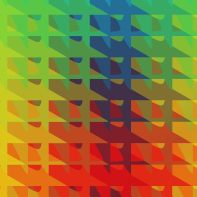
\includegraphics[width=.9\textwidth]{random_art/random_art1.jpg}
    \endminipage
    \minipage{0.32\textwidth}
        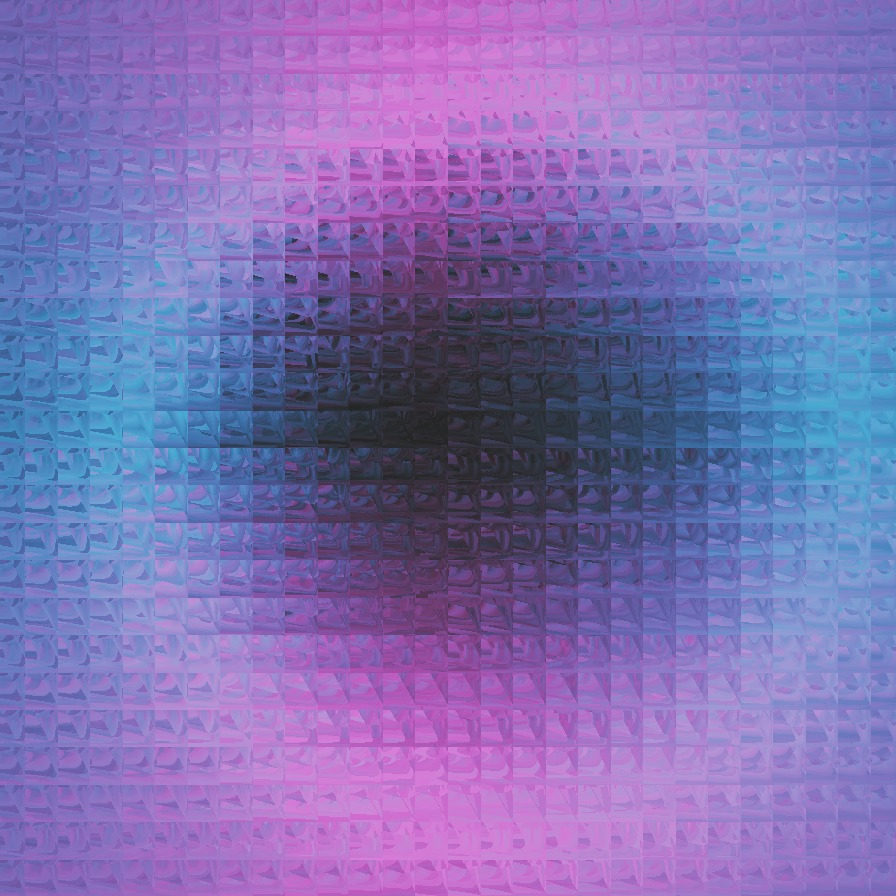
\includegraphics[width=.9\textwidth]{random_art/random_art2.jpg}
    \endminipage
    \minipage{0.32\textwidth}
        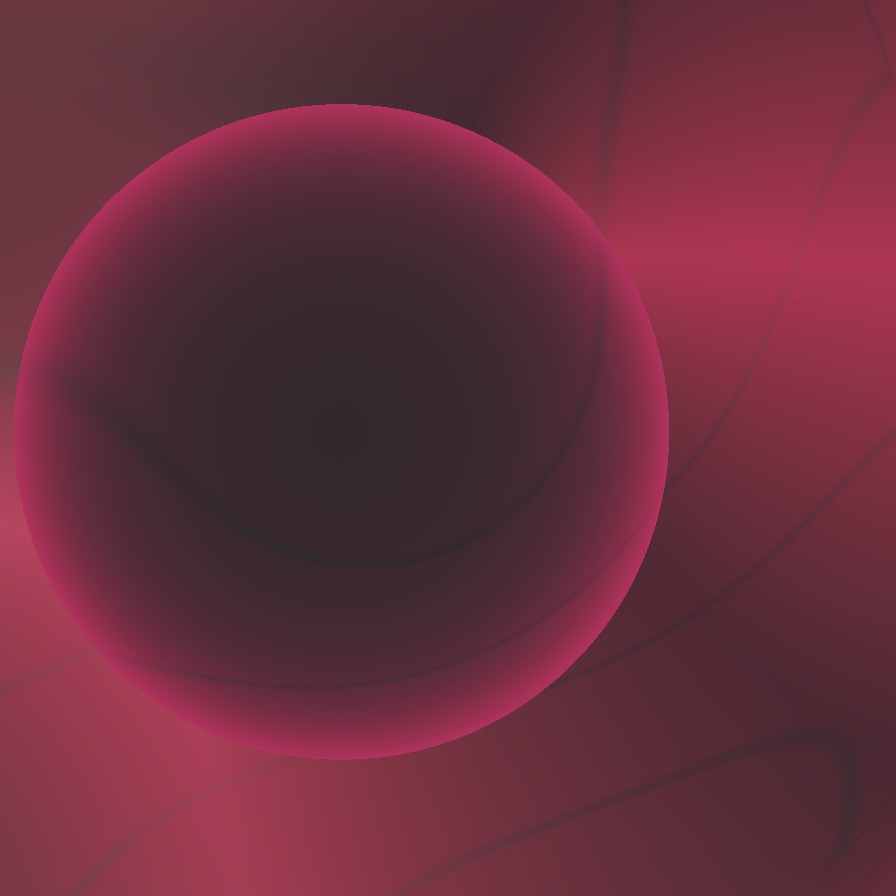
\includegraphics[width=.9\textwidth]{random_art/random_art3.jpg}
    \endminipage
    \caption{Random Art examples}
    \label{fig:randomArt}
\end{figure}

\textbf{Flag}. Flag is a visual hash scheme proposed by \textbf{C. Ellison} and \textbf{S. Dohrmann}\cite{ellison2003public}. Flag consists of four coloured strips with $2^n$ number of possible colours in each strip. 

\textbf{T-Flag}. T-Flag is an attempt to improve on the previously mentioned Flag \cite{lin2010spate}. Improvements include twice the number of coloured blocks with a choice of eight colourblind-proof colours.

\textbf{Flag-Ext}. Flag Extended is the proposed scheme assessed in the paper by \textbf{H. Hsiao \textit{et al.}}\cite{hsiao2009study}. Flag extended aims again, to improve on flag by reducing the number of blocks while adding 8 possible shapes.

Figure \ref{fig:flag} contains an example of each version of Flag discussed.

\begin{figure}[h!]
    \centering
    \minipage{0.32\textwidth}
        
\includegraphics[width=.9\textwidth]{flag/Flag.png}
        \caption{Flag}
    \endminipage
    \minipage{0.32\textwidth}
        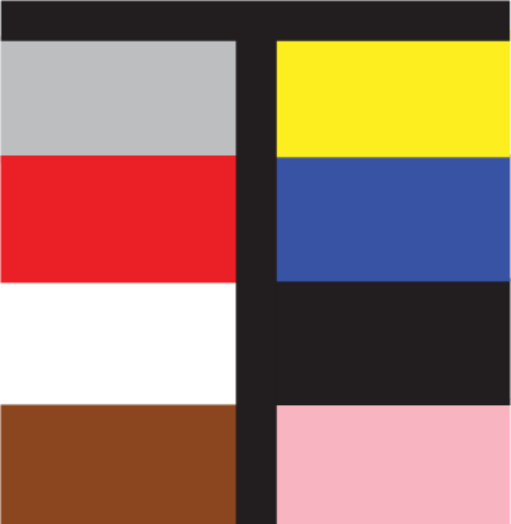
\includegraphics[width=.9\textwidth]{flag/T-Flag.png}
        \caption{T-Flag}
    \endminipage
    \minipage{0.32\textwidth}
        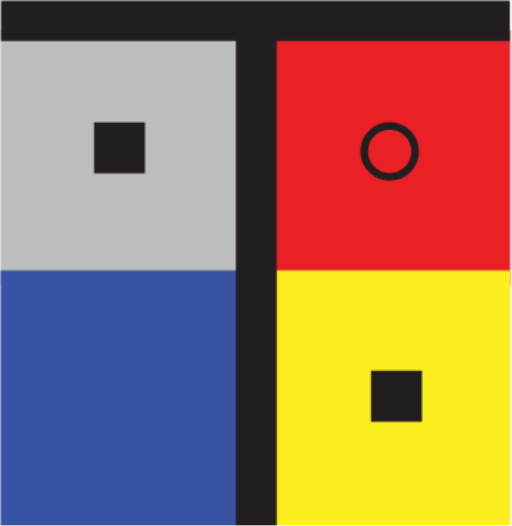
\includegraphics[width=.9\textwidth]{flag/Flag-ext.png}
        \caption{Flag Ext}
    \endminipage
    \caption{Variations of Flag}
    \label{fig:flag}
\end{figure}

\textbf{OpenSSH}. OpenSSH visual host key is an ASCII based graphical scheme used in MiTM detection when connecting to SSH servers. The image is generated by movement of the marker across a grid where every 2-bits of the generated MD5 has defines the diagonal direction of movement. For example, if the first 2-bits are \verb|11| the marker will move South East. The different characters are determined by the number of times the marker is present in that index, for example, if the maker is present on a square 4 times the character will be an equals sign (\verb|=|).

\textbf{Unicorns}\footnote{https://unicornify.pictures/}. Unicorns can be considered an example of an ``Avatar'' graphical scheme. The provided hash changes aspects of the image such as background colour, horn length and colour of the Unicorn's mane.

\textbf{Vash}\footnote{https://github.com/thevash/vash}. Vash is similar to that of unicorns where the hash determines certain characteristics of the image. Vash claims to have $\approx 5,438$ bits of entropy.

\begin{figure}[h!]
    \centering
    \minipage{0.32\textwidth}
        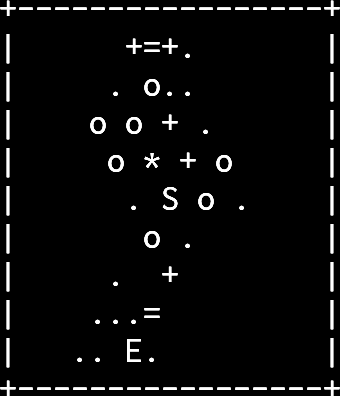
\includegraphics[width=.9\textwidth]{graphical/openssh.png}
        \caption{OpenSSH Visual Host Key}
    \endminipage
    \minipage{0.32\textwidth}
        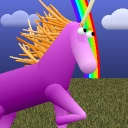
\includegraphics[width=.9\textwidth]{graphical/unicorn.png}
        \caption{Unicorn}
    \endminipage
    \minipage{0.32\textwidth}
        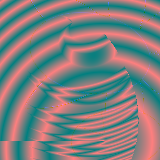
\includegraphics[width=.9\textwidth]{graphical/vash.png}
        \caption{Vash}
    \endminipage
    \caption{Examples of alternative graphical encoding schemes}
\end{figure}

Research in this area has taken these various encoding schemes and compared their fallibility to impersonated attacks. The main elements of comparison have been the ``accuracy of attack detection" and ``time to compare." In this paper, these are considered the metrics of ``security'' and ``usability,'' respectively.

\subsection{Similarity Metrics}
\label{sec:similarity_metric}
A similarity metric is an algorithm designed to determine if two words are phonetically a match. For example, the words "THEIR" and "THERE" is a match, whereas the words "DARK" and "PRINCIPLE" are not phonetically matching. This section provides a base explanation of important phonetic algorithms.

\subsubsection*{Soundex}
\label{sec:soundex}
One of the earliest examples of a phonetic algorithm is known as Soundex. It was initially designed for indexing names by phonetics alongside spelling mistakes due to transpositions in letters. 

Soundex produces a four-digit code for each word assessed.
The first letter of the word is retained alongside the removal of all of a, e, i, o, u, y, h and w. The remaining letters are then mapped to numbers. These mappings are displayed in Figure \ref{fig:soundexMap}.

\begin{figure}[h!]
    \centering
    \begin{BVerbatim}
b, f, p, v               1
c, g, j, k, q, s, x, z   2
d, t                     3
l                        4
m, n                     5
r                        6
    \end{BVerbatim}

    \caption{Soundex mappings of letters to numbers}
    \label{fig:soundexMap}
\end{figure}

Due to the fixed length and limited digit set the initial concerns from this design is the limited number of combinations. There are a total of 5616 codes due to 26 initial letters and three digits of 6 values ($26 * 6^3$).
The limited combinations result in matches of limited quality.

Further issues posed in \cite{patman2001soundex} are discussed below and show the further deficiencies of Soundex in a dictionary word matching context. 

\begin{enumerate}
    \item \textbf{Dependency on the first letter:} Soundex cannot match words together if their first letters are different, meaning, for example, the words "KORBIN" and "CORBIN" are considered non-matching. 

    \item \textbf{Silent consonants.} Soundex does not have logic embedded to deal with silent consonants.

    \item \textbf{Poor precision.} Due to the previously discussed point of a limited code space. \cite{patman2001soundex} re-iterates this point, but in the context of name matching where Soundex's poor performance was demonstrated. Soundex only gained and overall accuracy of 36.37\% when matching names within a provided database.
\end{enumerate}

\subsubsection*{NYSIIS}
\label{sec:nysiis}
The New York State Identification and Intelligence System (NYSIIS) phonetic code was created for use matching the phonetics of American names. The motivation for it's inception was mostly due to the presence of Hispanic names in the American based databases (this was an aspect Soundex was known to have low accuracy with). 

It also allows for variable-length codes and, thus, allows the applicability of the application to increase due to it not confronting the limited code issue of Soundex. It was in use right up util the end of 1998 within various US Government departments.

\subsubsection*{Metaphone}
\label{sec:metaphone}
Metaphone was invented by Lawrence Philips in 1990\cite{philips1990hanging} in response to the deficiencies in Soundex. It improves on Soundex by including information around inconsistency and variation in English spelling in an attempt to create a more accurate phonetic representation.

\subsubsection{Levenshtein Distance}
\label{sec:leven}
Levenshtein distance is a string metric designed to measure the `distance' between two strings. It is merely the number of single-character edits (insertions, deletions or substitutions) required to reach the other string.

An example distance between \verb|trace| and \verb|place| would be the substitutions of the first to letters, from \verb|tr| to \verb|pl|, meaning the two strings have a Levenshtein distance of 2.

\subsubsection{Phonetic Vectors}
\label{sec:phonetic_vectors}
Phonetic Vectors is a unique addition to the chosen set. Created by Allison Parrish in 2017\cite{parrish2017poetic}, Phonetic vectors is as the name suggests the vectorisation of the phonetics of a word.

Phonetic features are used in this work as a way to compare the similarity of phonemes. Phonemes are the phonetic elements that construct a word. For example, the word "RING" translated into the phonemes \verb|/R IH NG/|. 

Extensive prior work has gone into producing models of features that map to phonemes \cite{chomsky1968sound}\cite{ladefoged1969measurement}\cite{bradlow2010perceptual}. Features, therefore, are an attempt at mapping the varying and inconsistent rules around the pronunciation of the English language. The vectors were created using lists phonemes from the CMU Pronouncing Dictionary and mapping them to possible features.

\begin{table}[!htb]
    \tiny
    \begin{minipage}{.33\linewidth}
        \centering
        \begin{tabular}{ll}
            Phone & Features \\
            \hline
            AA & bck, low, unr, vwl \\
            AE & fnt, low, unr, vwl \\
            AH & cnt, mid, unr, vwl \\
            AO & bck, lmd, rnd, vwl \\
            AW & bck, cnt, low, rnd, smh, unr, vwl \\
            AY & cnt, fnt, low, smh, unr, vwl \\
            B & blb, stp, vcd \\
            CH & alv, frc, stp, vls \\
            D & alv, stp, vcd \\
            DH & dnt, frc, vcd \\
            EH & fnt, lmd, unr, vwl \\
            ER & cnt, rzd, umd, vwl \\
            EY & fnt, lmd, smh, unr, vwl
        \end{tabular}
    \end{minipage}%
    \begin{minipage}{.33\linewidth}
        \centering
        \begin{tabular}{ll}
            Phone & Features \\
            \hline
            F &  frc, lbd, vls \\
            G &  stp, vcd, vel \\
            HH & apr, glt \\
            IH & fnt, smh, unr, vwl \\
            IY & fnt, hgh, unr, vwl \\
            JH & alv, frc, stp, vcd \\
            K &  stp, vel, vls \\
            L &  alv, lat \\
            M &  blb, nas \\
            N &  alv, nas \\
            NG & nas, vel \\
            OW & bck, rnd, smh, umd, vwl \\
            OY & bck, fnt, lmd, rnd, smh, unr, vwl
        \end{tabular}
    \end{minipage} 
    \begin{minipage}{.33\linewidth}
        \centering
        \begin{tabular}{ll}
            Phone & Features \\
            \hline
            P & blb, stp, vls \\
            R & alv, apr \\
            S & alv, frc, vls \\
            SH & frc, pla, vls \\
            T & alv, stp, vls \\
            TH & dnt, frc, vls \\
            UH & bck, rnd, smh, vwl \\
            UW & bck, hgh, rnd, vwl \\
            V & frc, lbd, vcd \\
            W & apr, lbv \\
            Y & apr, pal \\
            Z & alv, frc, vcd \\
            ZH & frc, pla, vcd \\
        \end{tabular}
    \end{minipage} 
    \caption{Phonemes to feature mapping table}
    \label{tab:features}
\end{table}

Table \ref{tab:features} contains the mappings used in \cite{parrish2017poetic} to create the phonetic feature lists.
Using this with all 133,852 entries in version 0.7b of the CMU Pronouncing Dictionary, 949 unique properties were produced overall. The author then performed principal components analysis\footnote{Details regarding this process is outside the scope of the project. Please, however, if interested please refer to this resource for more information: \url{http://setosa.io/ev/principal-component-analysis/}} on the unique properties to reduce them down to 50.

This metric allows for a unique set of actions to be performed on the phonetic output. Not only does this metric allow the user to measure \textit{dissimilarity} (as opposed to the similar-or-not method of the alternatives) the continuous nature of the value allows mathematical operations to be performed on the output. An example shown in \cite{parrish2017poetic} was the addition of word vectors.

\begin{table}[!htb]
    \centering
    \begin{tabular}{cll}
        No & Operation & Result \\
        \hline
        1  & $Vec(\verb|sub|) + Vec(\verb|marine|)$ & \verb|submarine| \\
        2  & $Vec(\verb|miss|) + Vec(\verb|sieve|)$ & \verb|missive| \\
        3  & $Vec(\verb|fizz|) + Vec(\verb|theology|)$ & \verb|physiology| \\
    \end{tabular}
    \caption{Examples of vector addition}
    \label{tab:vectorAdd}
\end{table}

For example, the addition of vectors can be seen in Table \ref{tab:vectorAdd}. This works for any mathematical operation with examples like multiplication allowing the `tinting' words with a theme.



\section{Literature Review}
This section discusses the current research around the proposed topic.

The organisation of the section is as follows:

\begin{itemize}
    \item \textbf{Authentication ceremony performance} \\
    This section explains the current research on the performance of various encoding schemes and methods of comparison, alongside an assessment of the literature's experimental design.

    \item \textbf{Encoding schemes} \\
    The following section then discusses research around the design of an encoding scheme. The focus of the section is the technical details regarding the creation and design of schemes. 

    \item \textbf{Attacks on encoding schemes} \\
    The final section discusses literature that investigates the creation of actual attacks against encoding schemes.
\end{itemize}

\subsection{Authentication ceremony performance}

\subsubsection*{Encoding scheme performance}
Results 
from the literature consistently show the effectiveness of language-based encodings such as Words or Sentences with accuracies ranging up from 94\% \cite{dechand2016empirical}\cite{tan2017can}\cite{kainda2009usability}. In all cases, these were the best schemes from the sets assessed. The exception to this is the work performed by \textbf{H. Hsiao \textit{et al.}}\cite{hsiao2009study} in 2009 with Words achieving an abnormal accuracy of 63\%.
\\\\
Aside from textual representations were graphical schemes. As explained in Section \ref{sec:encodingSchemes} the main graphical schemes assessed by the literature were: Random Art, Flag, T-Flag, Vash, OpenSSH Visual Host Key and Unicorns. These schemes had mixed accuracy with ranges as large as 50\% - 94\% in work by \textbf{Hsiao \textit{et al.}}\cite{hsiao2009study}. The only other paper assessing graphical representations was the work of \textbf{Tan \textit{et al.}}\cite{tan2017can} where they also achieved mixed results with accuracies ranging from 46\% to 90\%.
\\
\begin{table}[h!]
    \makebox[\textwidth][c]{
        \begin{tabular}{c|ccccc}
    \toprule
    \textbf{Scheme} 
    & Hsu-Chun\cite{hsiao2009study}      
    & Kainda\cite{kainda2009usability}      
    & Dechand\cite{dechand2016empirical}
    & Tan\cite{tan2017can}      
    \\\hline
    Hexadecimal     &           &           & 11.20   & 9.00\\
    Numerical       &           & 6.00      & 10.60   & 9.00\\
    Base32          & 3.51      & 6.00      & 10.20   & \\
    Words           & 4.63      & 7.00      & 8.70    & 7.00 \\
    Scentences      &           & 11.00     & 12.30   & 8.00 \\
    Chinese Symbols & 5.01   &           &         & \\
    Japanese Symbols& 5.07   &           &         & \\
    Korean Symbols  & 4.92   &           &         & \\
    \midrule
    Random Art	     & 3.21   &&&&\\
    Flag    	     & 4.28   &&&&\\
    T-Flag  	     & 4.00   &&&&\\
    Flag Ext.	     & 4.02   &&&&\\
    OpenSSH`         &&&& 5.00 &\\
    Unicorns         &&&& 3.00 &\\
    Vash             &&&& 3.00 &\\
    \bottomrule
\end{tabular}
    }%
    \caption{Average comparison time (seconds) for the encoding schemes}
    \label{tab:times}
\end{table}
\\
In terms of usability of graphical schemes, the literature concurred on their high usability. The comparison speed of these schemes were all among the quickest (See Table \ref{tab:times} for an overview of timings). Other work also indirectly agreed with graphical encodings having significantly quicker comparison times compared to non-graphical schemes \cite{dechand2016empirical, kainda2009usability}.
In terms of research into the performance of graphical schemes, the literature does not contain an extensive review with literature only containing two papers. There is also no overlap in the schemes assessed with each paper reviewing a unique set. This area is, therefore, a promising candidate for further research.

One unique paper in this research area was the work by \textbf{M. Shirvanian, N. Saxena and J. J. George}\cite{shirvanian2017pitfalls} produced in the context of secure messaging pairing. This paper was unique for several reasons. First was to consideration for ``remote-vs-proximity'' pairing where this is the first consideration of this aspect found in the literature. There is room for further research to compare encoding schemes in the context of ``remote-vs-proximity.'' Another unique aspect was the end-to-end encryption context of the study.

The findings from the paper showed a high false-negative rate for all the schemes. This consideration is also missing from the literature. Alongside this, results for usability were lower in a remote setting for all the schemes. The author, however, comments on the expected nature of this result.\\
Images were identified as being the most secure method of authentication in the remote setting but voted as the method with the worst usability. This conclusion is highly inconsistent with all other work in this area. However, this could be due to the unique setting of remote verification, resulting in distinct results from user studies. Without further work in this area, it is difficult to validate these results conclusively.

Alongside this, it was shown in work by \textbf{H. Hsiao \textit{et al.}}\cite{hsiao2009study} that age and gender do not affect the accuracy of the scheme. However, younger participants were considerably faster. Furthermore, findings also showed that language comprehension helped in discerning small differences between schemes encoded in Chinese, Japanese, Korean, or English. Subsequently, knowledge of the language did not assist in differentiating more significant changes in the schemes as these had high accuracy regardless. These were unique considerations. Further work could aim to corroborate these conclusions.

\begin{table}[h!]
    \makebox[\textwidth][c]{
        \begin{tabular}{c|ccccc}
    \toprule
    \textbf{Scheme\footnote{All values have been rounded to the nearest whole percentage}} 
    & Hsu-Chun\cite{hsiao2009study}      
    & Kainda\cite{kainda2009usability}      
    & Dechand\cite{dechand2016empirical}
    & Tan\cite{tan2017can}      
    & M. Shirvanian\cite{shirvanian2017pitfalls}
    \\\hline
    Hexadecimal     &        &        & 90\% & 79\% &            \\
    Numerical       &        & 100\%  & 94\% & 65\% & 97\%       \\
    Base32          & 86\%   & ~~90\% & 92\% &      &            \\
    Words           & 63\%   & 100\%  & 94\% & 94\% &            \\
    Scentences      &        & 100\%  & 97\% & 94\% &            \\
    Chinese Symbols & 59\%   &        &      &      &            \\
    Japanese Symbols& 57\%   &        &      &      &            \\
    Korean Symbols  & 54\%   &        &      &      &            \\
    \midrule
    Random Art	     & 94\%   &&&&\\
    Flag    	     & 50\%   &&&&\\
    T-Flag  	     & 85\%   &&&&\\
    Flag Ext.	     & 88\%   &&&&\\
    OpenSSH`         &&&& 90\% &\\
    Unicorns         &&&& 46\% &\\
    Vash             &&&& 88\% &\\
    \bottomrule
\end{tabular}
    }%
    \caption{Overall accuracy of correct comparison for the encoding schemes assessed}
    \label{tab:results}
\end{table}

Tables \ref{tab:times} \& \ref{tab:results} contain the accuracy results of all papers assessed; this is to aid in visual comparison. Each paper used a different metric for measuring accuracy. Therefore, all results have been translated into ``overall accuracy.''. For example, if a paper presented "security failures" or "attack success rate" of 5\% the overall accuracy of the scheme is 95\%.

\subsubsection*{Methods of comparison performance}

Method of comparison is the way a user assesses the encoding scheme. The most common example and the one used as default is ``Compare-and-Confirm'' (CaC). CaC, as the name suggests, is the \textit{comparison} of two fingerprints on different devices or mediums that are then \textit{confirmed}. 

Aside from ``Compare-and-Confirm'' (CaC), there is ``Compare-and-Select'' (CaS) and ``Compare-and-Enter'' (CaE). CaS is the method where one device displays the fingerprint, and the other user is provided with several options. The user then has to choose the correct value from the list of candidates. If there is no match, the user must deny the connection attempt. The creation of CaS was due to concerns that CaC would be ``too easy'' for users leading to complacency and errors\cite{uzun2007usability}. The design of CaE is for scenarios where both devices might not have a display, i.e., pairing between a phone and a keyboard. One device displays the checksum. This checksum is then entered into the other device. The first device then compares the entered string and checks for a match.

Research has assessed the performance of these schemes and how they affect the security of the authentication ceremony. The literature agrees on CaC being the best overall scheme to compare fingerprints \cite{tan2017can}\cite{uzun2007usability} with CaS highlighted for its poor security and usability. CaE has had conflicting results. \cite{uzun2007usability} discarded it after one round due to ``poor usability.'' However, \cite{tan2017can} considered it the best method overall for usability and security. These conflicting results, therefore, show polarisation in the results of CaE. However, this could be due to the different overall use-cases of the studies. Validation of results from either study would, therefore, be an area of additional study.

\subsubsection*{Experimentation methodology comparison}
To further look into the validity of previously discussed results, it is necessary to asses how the respective studies reached their conclusions. Areas for consideration are scheme entropy, attacker strength, and participant demographics.

The starkest limitations of the literature are the range of participants and encoding entropy. The worst studies tested only 22-bits of entropy. This lack of entropy makes it challenging to compare results directly. One of the papers this most effects is the early work by \textbf{H. Hsiao \textit{et al.}}\cite{hsiao2009study}  where their highest entropy is 28-bits. This level of entropy was inadequate even at the time of publication. There is an attempt by the authors' to address this issue in the later stages of the paper where they write: \textit{``[...] increasing entropy is not a solution because it sacrifices usability and accuracy. With more entropy, representations will contain longer sequences of characters or more minute details which will lead to increased time and errors during comparisons.''}. This statement is backed up with no empirical evidence, and the authors fail to consider how the low entropy would affect the overall security of the schemes.

Attacker strength is also another metric used to compare results concluded by each paper. Some papers failed to address their attacker strength consideration directly, but the overall strength has been inferred from the changes made to their schemes. For example, if they decided to change a single character in a 40-digit (160-bit) SHA-1 hex digest, they are indirectly stating that the attacker can control 39-digits (156-bit). To achieve this, the attacker would have to compute $2^{156}$ SHA-1 compressions to find a key match.
In the literature, this element ranged from $2^{28}$ to around $2^{242}$. However, this has some relation to the size of the encoding schemes used. This substantial range makes it challenging to compare and confer results confidently. 
Further work could exclusively look into the effects that attacker strength has on the success of attacks. Moreover, all the papers assessed failed to fully consider the feasibility of attacks in terms of computer and storage requirements. 

All of the studies considered demographical data when presenting their results. Their average ages were all around $\sim35$ years old with the majority of participants educated with at least a bachelor degree. Alongside, the equal split between male and female participants.

One consideration of note is that made by \textbf{S. Dechand \textit{et al.}}\cite{dechand2016empirical} where they briefly consider medical conditions such as ADHD and reading or visual disorders and the way they affect the comparison's effectiveness. The results highlight a slight reduction in overall accuracy, however, due to their small sample size, the results cannot be considered conclusive. This aspect is unique to all literature assessed. Further work would be required to produce conclusive results. Therefore, highlighting a gap in the literature.

One glaring issue with the demographical health of the study by \textbf{E. Uzun, K. Karvonen} and \textbf{N. Asokan}\cite{uzun2007usability} is the use of two entirely different groups of participants. Not only were their demographics different, but they were from different countries (America and Finland). Different cultures contain inherent biases and assumptions. Changes were made pragmatically regarding the results from the first round of 40 participants. These were then re-assessed, alongside the direct comparison of results. This aspect casts vast doubts on the validity of the results with no consideration made by the authors to control external factors that may affect the performance of the method of comparison.

Hexadecimal and numerical schemes were not included as encoding schemes in work by \textbf{H. Hsiao \textit{et al.}}\cite{hsiao2009study} (some of the most widespread encoding schemes). The justification was the schemes similarities to Base32  alongside "well-known deficiencies". This point was provided with no further justification or quantified. Moreover, it is also inconsistent with available research, for example, in \textit{``Empirical Study of Textual Key-Fingerprint Representations''}\cite{dechand2016empirical} it was shown numerical representations performed significantly better than that of Base32.

\begin{table}[h!]
    \makebox[\textwidth][c]{
        \begin{tabular}{c|ccccc}
    \toprule
                        & Hsu-Chun\cite{hsiao2009study}      
                        & Kainda\cite{kainda2009usability}      
                        & Dechand\cite{dechand2016empirical}
                        & Tan\cite{tan2017can}      
                        & M. Shirvanian\cite{shirvanian2017pitfalls}
                        \\\hline
    Attacker Strength\footnote{Some attacker strengths are estimations due to the lack of quantification in some papers.}   
    & $\sim2^{28}$  & $\sim2^{40}$ & $2^{80}$ & $2^{60}$ & $\sim2^{242}$ \\
    Entropy Range       & 22-28 bits    & 20-40 bits   & 122 bits & 128 bits & 160-256 bits  \\
    No\degree  ~Participants     & 436           & 30           & 1047     & 661      & 25            \\
    \bottomrule
\end{tabular}
    }%
    \caption{Paper attribute comparison}
    \label{tab:attacker}
\end{table}

Table \ref{tab:attacker} has been provided to compare the different aspects of the papers' parameters visually. It can be seen from the table the substantial ranges in participant size, entropy and attacker strength.

\subsubsection*{Conclusion}
Overall, this review has identified several key areas suitable for further work.
The first is the performance assessment of graphical encoding schemes. Recreation of pre-existing results from \cite{hsiao2009study}\cite{tan2017can} is required to corroborate current conclusions and validate results.
Another gap in the research is the consideration into the utilisation of encoding schemes in realistic conditions, i.e. ``remove vs proximity." This topic was initially covered by \cite{shirvanian2017pitfalls}, but their scope was limited. Further work, therefore, could increase the scope and touch upon a large number of schemes in these settings. The final aspect for further work is the limited consideration into the feasibility of attacks on encoding schemes. All of the papers assessed simulated attacks and had minimal consideration for the execution of these attacks. Therefore, further work could delve
into the implementation and feasibility of such attacks.

\subsection{Encoding schemes}
Another area of research is investigations into the actual physical encodings of the hash digest. This section discusses the current research on the creation and security of actual encoding schemes. The technical details of the operation of the schemes are outside the scope of this literature review. Therefore, minimal attention is allocated to these details.

Some of the oldest preliminary work into visual encoding schemes is by \textbf{A. Perrig} and \textbf{D. Song}\cite{perrig1999hash} in the creation of their scheme ``Random Art" in 1999. The motivation for creating such a scheme was the perceived flaws in the ways humans verify and compare written information. As mentioned in previous sections, visual encoding schemes have been shown to have mixed success, with low security being one of their most alarming flaws. This research laid the foundation for further work in analysing the security of visual encoding schemes.

Further research into the creation of unique visual hash schemes has been performed by \textbf{C. Ellison} and \textbf{S. Dohrmann}\cite{ellison2003public} (Flag), \textbf{Yue-Hsun Lin \textit{et al.}}\cite{lin2010spate} (T-Flag) and work by \textbf{M.  Olembo \textit{et al.}}\cite{olembo2013developing}. Each publication has provided a new way  to represent a key fingerprint visually. Alongside the academic literature, there are informally presented methods of visual fingerprints such as Unicorns\footnote{https://unicornify.pictures/} and Robots\footnote{https://github.com/e1ven/Robohash}. This list is by no means exhaustive but is used to depict the amount of research and work invested into graphical hash representations.

One paper of note is the preliminary work performed by \textbf{D Loss \textit{et al.}}\cite{loss2009drunken} in their \textit{``An analysis of the OpenSSH fingerprint visualisation algorithm''} where  they aimed to spur on further research with their initial findings into the security of the OpenSSH scheme. The authors claim that the use of the algorithm in OpenSSH is only heuristically justified, and a more formal proof is required.\\
The paper proposed several ways to generate similar fingerprints. The methods proposed were: Naive brute force, Graph Theory, and brute force of a full visual set. They were only able to produce only initial results and have proposed a large amount of potential further work. Since the paper's publication in 2009, there seems to have been no research building on the work of the authors.

Minimal research has also focused on elemental textual fingerprint representations and their security. Work by \textbf{A. Karole} and \textbf{N. Saxena}\cite{karole2009improving} looked into ways to improve the security of a textual representation. This research aim was to improve the secure device pairing process of comparing two numerical values. The devices used (Nokia 6030b; Mid-range devices at the time of publication) and the SAS (Short Authentication String) compared results in findings that are not directly applicable in a fingerprint comparison context. 

A more specific subsection of textual fingerprints is the use of words and sentences to encode hash digests. Some of the first work in this area was by \textbf{Juola} and \textbf{Zimmermann} \cite{juola1996whole}. Their work aimed to produce a word list where phonetic distinctiveness was prioritised. Each word is mapped to a single byte. The unique aspect of the word list is the separation of ``even'' and ``odd'' words where ``even'' byte indices are sample from the even-list and ``odd'' from the odd-list. This technique effectively creates two sub-word lists.  A genetic algorithm was used to maximise linguistic distance. The paper also includes a study on effective measures of ``linguistic distances'' of words and provided an in-depth discussion into these areas.

Overall the paper provides a foundation for formalising the creation of effective wordlists. A limitation is the lack of empirical data gathered on the performance. However, this was later evaluated in work by \textbf{S. Dechand \textit{et al.}}\cite{dechand2016empirical} and shown to be an effective encoding scheme.

Other research of note is work by \textbf{M. Goodrich \textit{et al.}}\cite{goodrich2006loud} called \textit{Loud and Clear: Human-Verifiable Authentication Based on Audio}. As the name suggests, the authors were researching ways to improve current methods of secure device pairing. The unique aspect of this work is the use of a Text-to-Speech system reading out syntactically correct English sentences. MadLibs\footnote{https://en.wikipedia.org/wiki/Mad\_Libs} was the base for these sentences. MadLibs is where static placeholders are replaced with a list potential words.\\
This work is an extension to work performed by \textbf{Juola} and \textbf{Zimmermann}\cite{juola1996whole} as they aimed to emulate the techniques used in PGPfone. The paper's findings are limited by the lack of empirical data backing up claims made by the author the performance of the system, and security is only theoretically assessed.

Tanet alAside from this research, there have been further informal implementations of fingerprint encodings. The first being by \textbf{Michael Rogers}\footnote{https://github.com/akwizgran/basic-english}. Rogers' implementation is a program designed to map fingerprints to pseudo-random poems. This implementation was again, empirically evaluated by \textbf{S. Dechand \textit{et al.}}\cite{dechand2016empirical}. Ealier work by \textbf{N. Haller} with the S/KEY\cite{haller1995s} shows the implementation of a system designed to represent a hash as a series of six short words. However, this system is designed for a one-time-password purpose and only provides word mappings for basic human usability of the password and not within a fingerprint verification context. Therefore, the wordlist has not been designed with pronounceability in mind.

\newpage
\subsubsection*{Pretty Easy Privacy}
\label{sec:pep}
A very recent implementation of a word list can be found in Pretty Easy Privacy (\pep) implementation of TrustWords\footnote{https://tools.ietf.org/html/draft-birk-pep-trustwords-03}. \pep is a data encryption system that utilises PGP encryption to provide E2EE on all common channels of communication such as email or SMS. The embedded design principles state that above all the systems should be easy to install, use and understand.

\begin{wrapfigure}{r}{6cm}
    \centering
    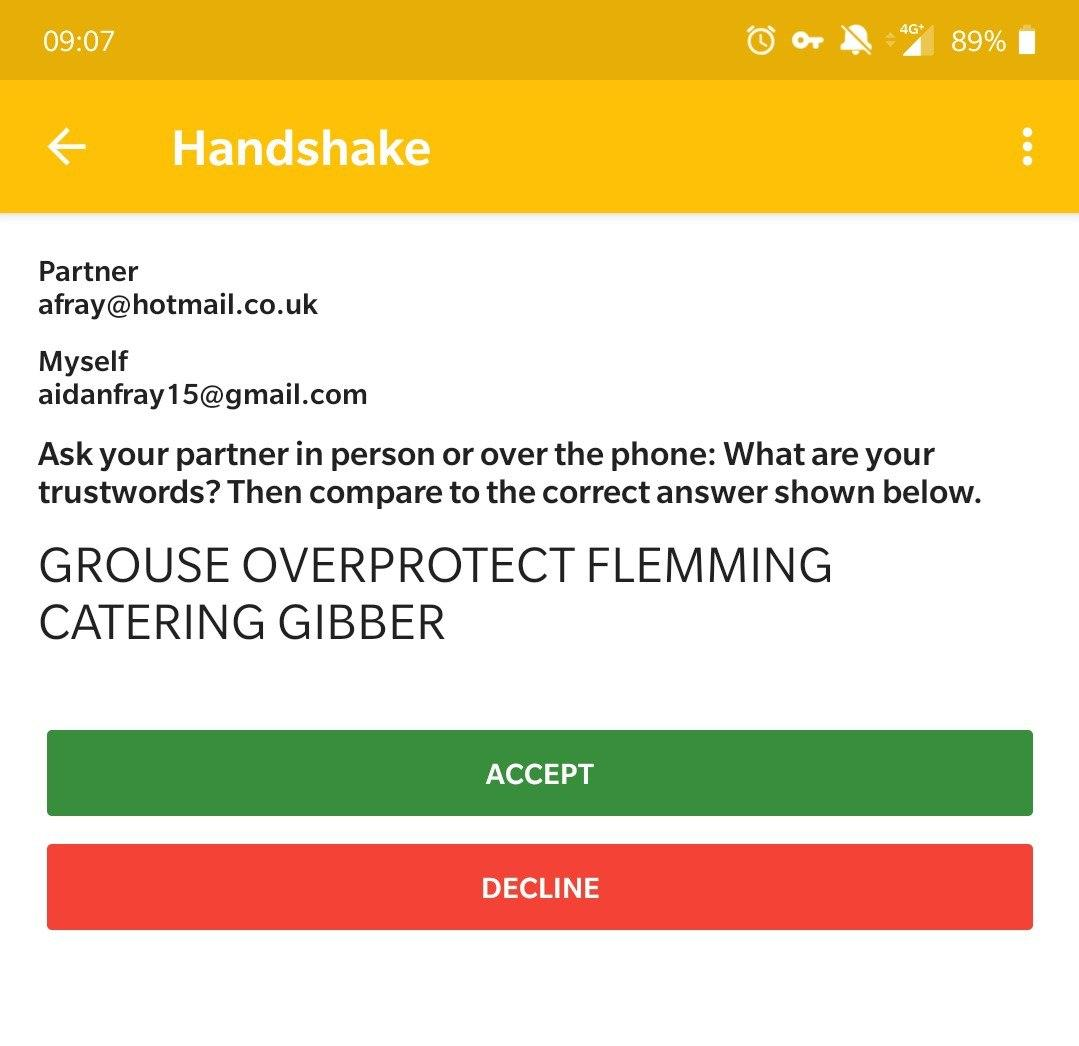
\includegraphics[scale=0.15]{trustwords/trustword_handshake.jpg}
    \caption{Trustword fingerprint verification}
    \label{fig:trustwords}
\end{wrapfigure}

\pep deals with the threat of MiTM attacks by having users compare the respective key fingerprints encoded as a set of words. Figure \ref{fig:trustwords} shows the \pep Android implementation of Trustwords. The users then authenticate the words on an OOB (Out of Band) channel such as a phone call or in-person communication. If both users decide the words match, they accept or decline respectively.

The unique aspect of TrustWords is its mapping of a single word to 16-bits. If compared to alternative literature, this is the highest number of bits-per-word seen. Full mappings (no duplication of words) would, therefore, require $2^{16}$ words in the dictionary. This number of words is arguably higher than most users' vocabulary. This deviation from the norm has not been currently backed up by research. 

\begin{wrapfigure}{l}{5cm}
    \centering
    \begin{BVerbatim}
    [...]
52127 ZYGOTE
52128 ZYGOTIC
52129 ZYMURGY
52130 AACHEN
52131 AARDVARK
52132 AAREN
    [...]
    \end{BVerbatim}
    \caption{Re-mapping position in Trustword dictionary}
    \label{fig:remap}
\end{wrapfigure}

Alongside the abnormally high number of words, the design choice to exclude slang and profanities from the English Trustword dictionary requires dual-mapping of a section of words. Approximately 13633/65536 (20.8\%) of words are re-mapped in the dictionary, leaving 51903 unique words. The re-mapping looped with the dictionary remaining alphabetical. Figure \ref{fig:remap} shows the position in the dictionary where this occurs.

Moreover, the primary RFC documentation remains in a draft stage and states: \textit{``It is for further study, what minimal number of words (or entropy) should be required.''}. These aspects highlight a substantial gap in the current literature.

\subsubsection*{Conclusion}

In conclusion to this topic, the current research has primarily focused on the research and creation of visual representations. Research for textual fingerprints is fragmented and incomplete with work \textbf{Juola} and \textbf{Zimmermann} 
\cite{juola1996whole} and \textbf{M. Goodrich \textit{et al.}}\cite{goodrich2006loud} providing meaningful research to build upon in terms of word and sentence based encodings. The fragmentation of this research leaves room for further work into this topic area. Alongside this, findings from the previous section's research show that human language based encodings provided the best usability and, therefore, should be a target for further research looking to improve upon their security and usability.

\subsection{Attacks on encoding schemes}
This area of research studies ways to physically execute attacks on fingerprint encoding schemes. This topic differs from previously examined work due to papers discussing the performance and fallibility of encoding schemes simulated the attack without consideration for how the attack execution. Research in this area is scant, with lots of research attention on security of Man-in-the-Middle (MITM) attacks and not the encoding schemes themselves.

Research in 2002 by \textbf{Konrad Rieck}\cite{rieck2002fuzzy} is one the first formalisation of attacks on fingerprint representations. The paper titled \textit{``Fuzzy Fingerprints Attacking Vulnerabilities in the Human Brain''} aimed to look into ways users check hexadecimal encoded OpenSSH fingerprint representations. The author created an elegant way to `weight' essential chunks of the digest. The bytes furthest to the right and left of the digests provided the highest weight. This technique provides a way to score digests and determine the best partial collisions found. For example, with the target fingerprint: \verb|9F23| and partial match \verb|9313| is given a score of 45\% even though only two characters are matching.

The paper contains an implementation with a ``1.2GHz CPU'' being able to obtain 130,000 H/s (With MD5). In comparison to this, a mid-range Intel i5-3320M CPU can today obtain 111,700,000 MD5 H/s. This imbalance shows that the results obtained from the paper are significantly outdated. However, even with the low hash rate, the author was able to obtain some promising results. Figure~\ref{ref:fuzz} contains the best example used.

\begin{figure}[!h]
    \begin{center}
        \verb|TARGET: d6:b7:df:31:aa:55:d2:56:9b:32:71:61:24:08:44:87|
        \verb|MATCH:  d6:b7:8f:a6:fa:21:0c:0d:7d:0a:fb:9d:30:90:4a:87|
    \end{center}
    \caption{Best match obtained after a few minutes of hashing}
    \label{ref:fuzz}
\end{figure}

Overall the paper shows an interesting way to create partial fingerprint matches but is not quantified by any empirical evidence gathered on real-world users. 

The only other relevant research on this topic is the work by \textbf{M Shirvanian and N. Saxena}\cite{shirvanian2014wiretapping} 
and their paper: \textit{``Wiretapping via Mimicry: Short 
Voice Imitation Man-in-the-Middle Attacks on Crypto 
Phones''}. Further research in the area of ``human voice impersonation'' has received lots of attention \cite{mukhopadhyay2015all}\cite{chen2017you}\cite{wu2015spoofing}. This paper was chosen over other alternatives due to its specific use of encoding schemes in its evaluation.

In this paper, the authors develop a way to 
impersonate users when authenticating 
Short-authentication-Strings (SAS) in the pairing of 
Crypto-phones. To achieve this impersonating they propose 
two methods: ``Short voice re-ordering attack'' where an 
arbitrary SAS string is recreated by re-ordering snipped 
obtained from eavesdropping a previous connection
and ``Short voice morphing attacks'' whereby the use of 
previously eavesdropped audio snippets the attacker can
morph their voice to match that of the victim. With 
these methods, they aimed to attack encodings of Numbers, 
PGP word list (previously discussed work by \textbf{Juola} and 
\textbf{Zimmermann} \cite{juola1996whole}) and MadLib (\textbf{M. Goodrich 
\textit{et al.}}\cite{goodrich2006loud} work also 
previously discussed). The effectiveness of these attacks 
was evaluated with a study involving 30 participants.

Results from the paper show the effectiveness of these 
methods. Compared to the baseline of the attacker's voice 
replacing the victim, performed with an $\sim$18\% success rate. Morphing gained an overall success rate of 50.58\% and re-ordering a very impressive 78.23\% success rate and showing that these attacks provide an improvement on top of the naive implementation.

One of the most significant limitations addressed by the authors  was the reduction in success rates as the size of the authentication string grew. The morphing and re-ordering  attacks become increasingly ineffective as the user had more time to detect imperfections. This aspect is not quantified by the author and the extent of this degradation is never empirically discussed. Therefore, the results from this study are only effective and applicable in a SAS context.

\subsubsection*{Topic Conclusion}
Overall the literature for this subtopic remains sparse and incomplete. Further suggested work could look into the feasibility of generating partial collisions for all textual representations alongside quantified effectiveness on users. With the possibility to concentrate on a few selected implementations. The work would aim to focus on the various physical methods used and their feasibility. This is one area the previous literature has failed to cover and has only theoretically quantified attacker strength without consideration for the actual real-world cost of these attacks.

\section{Overall Summary}
In summary of the literature gaps areas discovered; encoding scheme performance requires further work in the performance of all graphical schemes to back up the results made by other work. Furthermore, there is a gap with the assessment of encoding schemes in the context of "remote-vs-proximity" first proposed by \textbf{M. Shirvanian, N. Saxena} and \textbf{J. J. George}\cite{shirvanian2017pitfalls} as it would arguably provide a better simulation of real-world scenarios.

In the context of human demographics and the way they alter the performance of the schemes; further research is required into how the fluency of languages affects authentication ceremony. This further work would be a continuation of the initial work by \textbf{H. Hsiao \textit{et al.}}\cite{hsiao2009study} and could allow the creation of schemes that are better suited to specific languages.
Alongside this, there is a research gap in the investigation of how mental impairments affect the performance. This aspect is useful due to the number of potential users being affected due to systems not being designed with them in mind. For example, 7\% of the population have been identified as having dyslexic tendencies\cite{peterson2012developmental}. This fact means that with a UK population of around 63,000,000\footnote{From the 2011 Census collated by the Office for National Statistics}  4,410,000 people could benefit from encoding schemes designed to work well with dyslexia. Dyslexia, however, is only one of many impairments that could affect a scheme's performance, thus further contributing to the substantial effect further work could have on this area.

Other possible large areas for consideration is the lacks of direct consideration for attack strength when assessing the vulnerability of encoding schemes. Issues included the previously discussed wide range of attack strength ($2^{28}$ - $2^{242}$) alongside the lack of consideration at all from the majority of papers. Moreover, the complete lack of computation and storage complexity considerations means this is a prime area for further research as it would improve the applicability of results.

The final significant research gap identified is the lack of justification for the newly created Trustwords. Abnormal design choices (16-bit per word) and its recent creation alongside the shown effectiveness of language-based encodings, such as words makes this a promising area for further research. 